%!TEX root = ../aistats_paper.tex
\section{Experiments}
\label{sec:experiments}

We implemented both minibatch approaches in PyTorch, and compared against the reference implementation from \citet{bovyExtremeDeconvolutionInferring2011}.
To evaluate each method, we used a random sample of rows from the Gaia DR2 source table~\cite{brownGaiaDataRelease2018}.
We selected the 5 primary astrometric features, along with the BP-RP colour and mean magnitude in the G-band.
In total there were 2 million rows.
Where data were missing, we set the field to zero and the noise variance to a large value.
We set the projection $R_i$ to the identity matrix for every sample.
This preliminary study uses only a small fraction of the full dataset size, but this allows us to fit the training data into memory, a requirement for use with the original implementation of extreme deconvolution.
We used a range of mixture component sizes $K$.
In practice we would want to select a value of $K$ by cross-validation.

The existing EM method ran on CPU, whilst the minibatch EM and SGD methods ran on GPU\@.
While the absolute times depend strongly on hardware and fine implementation details, they give a sense of the sort of times possible on current workstations, and the relative times across model sizes illustrate how the methods scale.
We used a validation set comprising $10\%$ of the rows when developing our experiments.
Final model performance was evaluated on a different held-out test set also comprising 10\% of the rows at the last stage, with no parameter selection or development done based on this set.

Table~\ref{results-table} reports the validation and test log-likelihoods for each method.
The values are similar, but not exactly comparable, as the effect of regularisation differs for each method.
Figure~\ref{fig:training} plots the training log-likelihood against time-rescaled epoch for $K=256$, and training time as function of mixture components $K$.
Figure~\ref{fig:projection} shows a 2-D projection from an example model with $K=256$ fitted with the minibatch-EM method.

\begin{table*}{}
  \caption{Average validation log-likelihoods for the Gaia data subset for different numbers of mixture components $K$, with average test log-likelihood for the best value of $K$ by validation. Average over 10 runs with standard deviation.}
  \label{results-table}
  \centering
  \begin{tabular}{lcccc}
      \toprule
      Method     & K &  Validation     & Test\\
      \midrule
      Existing EM & 64 & $-26.10 \pm 0.03$ & - \\
      \citet{bovyExtremeDeconvolutionInferring2011} & 128 & $-25.96 \pm 0.04$ & - \\
       & 256 & $-25.76 \pm 0.02$ & - \\
       & 512 & $-25.67 \pm 0.01$ & $-25.66 \pm 0.01$ \\
      \midrule
      Minibatch EM & 64 & $-26.05 \pm 0.01$ & - \\
       & 128 & $-25.91 \pm 0.01$ & - \\
       & 256 & $-25.83 \pm 0.00$ & - \\
       & 512 & $-25.80 \pm 0.00$ & $-25.79 \pm 0.00$ \\
      \midrule
      SGD & 64 & $-25.89 \pm 0.02$ & - \\
       & 128 & $-25.77 \pm 0.02$ & - \\
       & 256 & $-25.67 \pm 0.02$ & - \\
       & 512 & $-25.59 \pm 0.02$ & $-25.57 \pm 0.02$ \\
      \bottomrule
  \end{tabular}
\end{table*}

\begin{figure*}
  \centering
  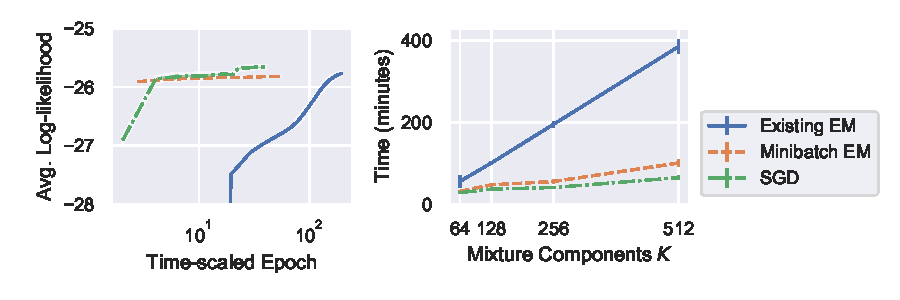
\includegraphics[width=\textwidth]{figures/learning.pdf}
  \caption{\textbf{Left}: Average training log-likelihood as a function of training epoch for models with $K=256$. Epochs rescaled by average training time. Error bars not visible. \textbf{Right}: Training time as a function of mixture components $K$. Error bars indicate $\pm$ 2 standard deviations.}
  \label{fig:training}
\end{figure*}

\begin{figure*}
  \centering
  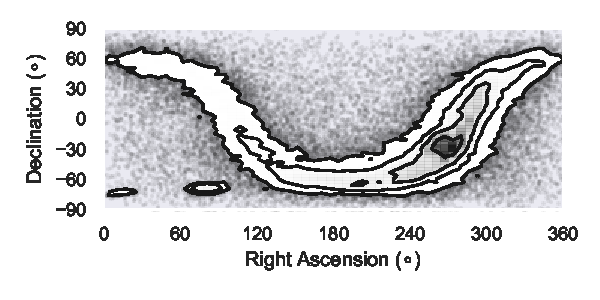
\includegraphics{figures/density.pdf}
  \caption{Density plot showing a 2-D projection of 100000 samples drawn from a model with $K=256$ and fitted with the minibatch EM method.
  The plot shows the estimated density of star positions on the sky, and has correctly recovered the structure of the Milky Way and the Magellanic Clouds.}
  \label{fig:projection}
\end{figure*}
